\documentclass{beamer}
\usetheme[
  block=fill,
  background=dark,
  titleformat=smallcaps,
  progressbar=frametitle,
  numbering=none,
]{metropolis}

%----------------------------------------------------------------------------
% LoCo
%----------------------------------------------------------------------------
\setbeamertemplate{frametitle}[default][center]
\newcommand{\xx}{\pmb{\raisebox{-1.5pt}{$\mathcal{X}$}}}
\newcommand{\hh}{\pmb{h}}
\newcommand{\ii}{\pmb{i}}
\newcommand{\oo}{\pmb{o}}
\newcommand{\ff}{\pmb{f}}
\newcommand{\Ss}{\pmb{s}}
\newcommand{\Cc}{\pmb{c}}
\newcommand{\bb}{\pmb{b}}

%Color
\definecolor{mDarkBrown}{HTML}{604c38}
\definecolor{mDarkTeal}{HTML}{23373b}
\definecolor{mLightBrown}{HTML}{EB811B}
\definecolor{mLightGreen}{HTML}{14B03D}
% Math
\usepackage{amsmath}
\usepackage{amssymb}
\usepackage{stmaryrd}
\usepackage{bm}
\newenvironment{rcases}
  {\left.\begin{aligned}}
  {\end{aligned}\right\rbrace}

% Code listing
\usepackage{minted}
%\usemintedstyle{friendly}
\usemintedstyle{tango}
\usepackage{algorithm}
\usepackage[noend]{algpseudocode}

% Graphs
\usepackage{tikz}
\usetikzlibrary{calc, trees, fit, positioning}
\usepackage{pgfplots}
% Graphics
\usepackage{graphics}
\graphicspath{{figures/}} % Location of the graphics files

\newcommand\todo[1]{\textcolor{red}{#1}}
\newcommand{\w}[1]{\textit{"#1"}}
\newcommand{\sm}[1]{\text{\small{#1}}}

% Box macro
\newcommand{\ex}[2]{
  \vfill
  \begin{alertblock}{#1}
    #2
  \end{alertblock}
}
\newcommand\tsc[1]{\alert{\textsc{#1}}}

%----------------------------------------------------------------------------

% Beamer
\title{Differentiable Neural Computers}
\subtitle{Hybrid Computing using a neural network with dynamic external memory (Graves et al. 2016)}
\author{Konstantinos Kogkalidis}
\date{May 28, 2018}
\institute{Logic and Computation}

\begin{document}
	\maketitle
	
\begin{frame}{Overview: Probabilistic Programming}
	\alert{Cross-domain}
	\begin{itemize}
	\item Data Flow Programming
	\item Bayesian Reasoning / Machine Learning
	\item Fuzzy Logic
	\item Functional Programming
	\end{itemize}
	\pause
	Intuition:
	\textit{"Rather than explicitly write a program, write some \alert{constraints} on the behavior of the desired program and use computational tools to search the program space for \alert{models} satisfying these constraints."}
	\pause
	\[\begin{array}{rcl}
	\textsc{\alert{Program}} &\ & \textsc{\alert{Model}}\\
	\hline
	\text{Discrete} &\ & \text{Continuous}\\
	\text{Deterministic} &\ & \text{Stochastic}\\
	\text{Static} &\ & \text{Adaptive}\\
	\end{array}\]
\end{frame}

\begin{frame}{Overview: DNC}
	\alert{Differentiable Neural Computer}\\
	A recurrent neural network coupled with an external memory.
	
	\pause
	\begin{itemize}
	\item Functional replication of biological memory
	\item Reimaging of classical concepts of computation
	\item Extension of NTMs
	\begin{itemize}
		\item End-to-end differentiable
		\item Auto-associative memory
		\item Turing complete
		\item[+] Computationally efficient memory management
	\end{itemize}
	\end{itemize}
\end{frame}

\begin{frame}{Introduction: Classic Computation}
	\alert{Von Neumann architecture}
	\begin{figure}
	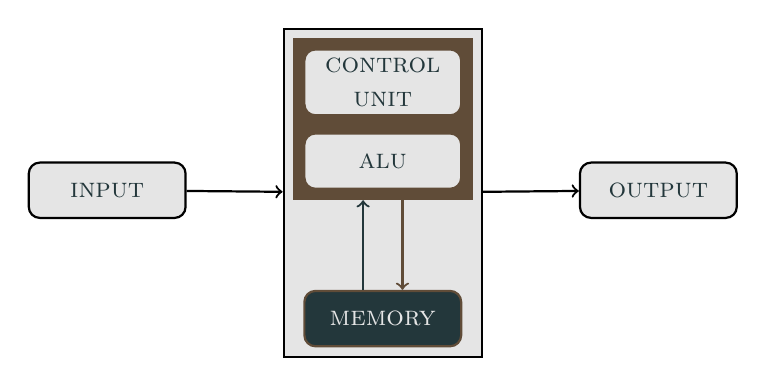
\begin{tikzpicture}
		[auto,
		block/.style ={rectangle, draw=mDarkBrown, thick, fill=gray!20, text width=5em, align=center, rounded corners, minimum height=2em},
		block2/.style ={rectangle, draw=mDarkBrown, thick, fill=mDarkTeal, text width=5em, align=center, rounded corners, minimum height=2em},
		block3/.style ={rectangle, draw=black, thick, fill=gray!20, text width=5em, align=center, rounded corners, minimum height=2em}]
		\draw (-1,0.63) node[block3] (i) {\textcolor{mDarkTeal}{\sc{input}}};
		\draw (6,0.63) node[block3] (o) {\textcolor{mDarkTeal}{\sc{output}}};
		
		\draw (2.5,-1) node[block2] (m) {\textcolor{gray!20}{\sc{memory}}};
		\draw (2.5,1) node[block] (a) {\textcolor{mDarkTeal}{\sc{alu}}};
		\draw (2.5,2) node[block] (c) {\textcolor{mDarkTeal}{\sc{control unit}}};
		
		\node[draw=mDarkBrown, thick, fill=mDarkBrown, fit=(a) (c)](Fit1) {};
		\draw (2.5,1) node[block] (a) {\textcolor{mDarkTeal}{\sc{alu}}};
		\draw (2.5,2) node[block] (c) {\textcolor{mDarkTeal}{\sc{control unit}}};
		
		\node[draw=black, thick, fill=gray!20, fit=(Fit1) (m)](Fit2) {};
		\node[draw=mDarkBrown, thick, fill=mDarkBrown, fit=(a) (c)](Fit1) {};
		\draw (2.5,1) node[block] (a) {\textcolor{mDarkTeal}{\sc{alu}}};
		\draw (2.5,2) node[block] (c) {\textcolor{mDarkTeal}{\sc{control unit}}};
		\draw (2.5,-1) node[block2] (m) {\textcolor{gray!20}{\sc{memory}}};

		\draw (i) edge [->, black, thick] (Fit2);
		\draw (Fit2) edge [->, black, thick] (o);
		\draw ($(m.north) + (0.25,0)$) edge [<-, mDarkBrown, thick] ($(Fit1.south) + (0.25, 0)$ );
		\draw ($(m.north) + (-0.25,0)$) edge [->, mDarkTeal, thick] ($(Fit1.south) + (-0.25, 0)$ );

	\end{tikzpicture}
	\end{figure}
\end{frame}

\begin{frame}{Introduction: Neural Networks}
	\begin{minipage}[t]{.44\textwidth}	
	\alert{Simple Neural Net}
	\begin{figure}[h!]
	\vspace{6.5pt}
	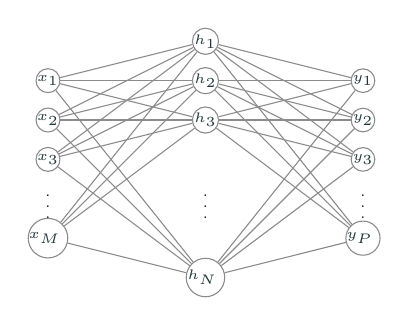
\begin{tikzpicture}[scale=.5]
		\foreach \y /\alph/\name in {
			0/x1/$x_1$,
		  	-1/x2/$x_2$,
		  	-2/x3/$x_3$,
		  	-4/xM/$x_M$
		 }{
		 	\node[circle, draw=gray!90, inner sep=0pt,minimum size=3mm,fill=white] (\alph) at (0,\y) {\tiny \textcolor{mDarkTeal}{\name}};
		 }
		 \node (x..) at (0,-3) {\tiny {\vdots}};
		 \foreach \y /\alph/\name in {
			1/h1/$h_1$,
		  	0/h2/$h_2$,
		  	-1/h3/$h_3$,
		  	-5/hN/$h_N$
		 }{
		 	\node[circle, draw=gray!90, inner sep=0pt,minimum size=3mm,fill=white] (\alph) at (4,\y) {\tiny \textcolor{mDarkTeal}{\name}};
		 }
		 \node (h..) at (4,-3) {\tiny {\vdots}};
		 \foreach \y /\alph/\name in {
			0/y1/$y_1$,
		  	-1/y2/$y_2$,
		  	-2/y3/$y_3$,
		  	-4/yP/$y_P$
		 }{
		 	\node[circle, draw=gray!90,inner sep=0pt,minimum size=3mm,fill=white] (\alph) at (8,\y) {\tiny \textcolor{mDarkTeal}{\name}};
		 }
		 \node (y..) at (8,-3) {\tiny {\vdots}};
		 \foreach \x in {x1, x2, x3, xM}
		 {\foreach \h in {h1, h2, h3, hN}
		 {\draw (\x) edge[gray!90] (\h);}}
		 \foreach \x in {h1, h2, h3, hN}
		 {\foreach \y in {y1, y2, y3, yP}
		 {\draw (\x) edge[gray!90] (\y);}}
	\end{tikzpicture}
	\end{figure}
	\vspace{10pt}
	\centering
	%\small \alert{$y=g(h),\ h=f(x)$}\\
	\small $NN: \pmb{x}_{t} \mapsto \pmb{y}_{t}$\\
	\alert{No memory}
	\end{minipage}
	\pause
	\hspace{1cm}
	\begin{minipage}[t]{.44\textwidth}	
	\alert{Simple Recurrent Net}
	\begin{figure}[h!]
	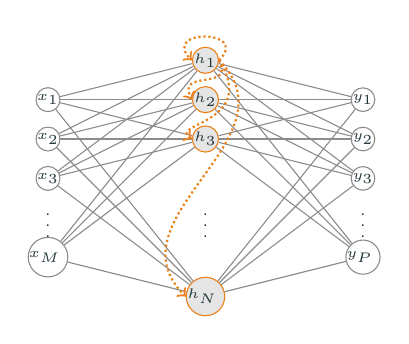
\begin{tikzpicture}[scale=.5]
		\foreach \y /\alph/\name in {
			0/x1/$x_1$,
		  	-1/x2/$x_2$,
		  	-2/x3/$x_3$,
		  	-4/xM/$x_M$
		 }{
		% 	\node[] (\alph) at (0,\y) {\name};
		 	\node[circle, draw=gray!90, inner sep=0pt,minimum size=3mm,fill=white] (\alph) at (0,\y) {\tiny \textcolor{mDarkTeal}{\name}};
		 }
		 \node (x..) at (0,-3) {\tiny {\vdots}};
		 \foreach \y /\alph/\name in {
			1/h1/$h_1$,
		  	0/h2/$h_2$,
		  	-1/h3/$h_3$,
		  	-5/hN/$h_N$
		 }{
		 	\node[circle, draw=mLightBrown, inner sep=0pt,minimum size=3mm,fill=gray!20] (\alph) at (4,\y) {\tiny \textcolor{mDarkTeal}{\name}};
		 }
		 \node (h..) at (4,-3) {\tiny {\vdots}};
		 \foreach \y /\alph/\name in {
			0/y1/$y_1$,
		  	-1/y2/$y_2$,
		  	-2/y3/$y_3$,
		  	-4/yP/$y_P$
		 }{
		 	\node[circle, draw=gray!90, inner sep=0pt,minimum size=3mm,fill=white] (\alph) at (8,\y) {\tiny \textcolor{mDarkTeal}{\name}};
		 }
		 \node (y..) at (8,-3) {\tiny {\vdots}};
		 \foreach \x in {x1, x2, x3, xM}
		 {\foreach \h in {h1, h2, h3, hN}
		 {\draw (\x) edge[gray!90] (\h);}}
		 \foreach \x in {h1, h2, h3, hN}
		 {\foreach \y in {y1, y2, y3, yP}
		 {\draw (\x) edge[gray!90] (\y);}}
		 \draw (h1.east) [->, densely dotted, thick, mLightBrown] .. controls +(0.8,0.8) and +(-0.8,0.8) .. (h1.west);
		 \draw (h1.east) [->, densely dotted, thick, mLightBrown] .. controls +(0.4,-0.8) and +(-0.4,0.8) .. (h2.west);
		 \draw (h1.east) [->, densely dotted, thick, mLightBrown] .. controls +(1,-1.6) and +(-0.6,0.4) .. (h3.west);
		 \draw (h1.east) [->, densely dotted, thick, mLightBrown] .. controls +(2,-2) and +(-2,2) .. (hN.west);
	\end{tikzpicture}
	\end{figure}
	\vspace{10pt}
	\centering
	%\small{ \alert{$h(t)=f([x(t); h(t-1)])$}}\\
	\small{ $RNN: \pmb{x}_{0} \otimes \pmb{x}_{1} \otimes \dots \otimes \pmb{x}_{t} \mapsto \pmb{y}_{t}$}\\
	\alert{Finite memory}
	\end{minipage}
	\pause
	
	\begin{quote}
	\small \textit{"If training vanilla neural nets is optimization over functions, training recurrent nets is \alert{optimization over programs}."}
	\end{quote}
\end{frame}

\begin{frame}{Approach}
	Train a RNN to act as the \alert{controller} of a memory matrix $M \in \mathbb{R}^{N\times W}$ through R \alert{read heads} and one \alert{write head}.
	
	\pause
	\begin{enumerate}
	\item \alert{Content Lookup}\\
		\begin{itemize}
		\item \alert{Attention} over memory defined by weightings $w \in \mathcal{S}^N$
		\item Compare controller output with memory objects (\alert{auto-associative memory})
		\item Allow partial matches  (\alert{pattern completion})
		\end{itemize}
	\pause
	\item \alert{Sequential Retrieval}
		\begin{itemize} 
		\item Fill $L \in [0,1]^{N \times N}$ indexing \alert{temporal transitions}
		\item \alert{Shift} operations defined by $Lw,\ L^\top w$
		\end{itemize}
	\pause
	\item \alert{Dynamic Allocation}
		\begin{itemize}
		\item Mark memory locations with $\pmb{u} \in [0,1]^N$ to \alert{signal usage}
		\item Manipulate signals during R/W operations to enable \alert{reallocation}
		\item Generalization to \alert{unbounded memory}
		\end{itemize}
	\end{enumerate}
\end{frame}
	
\begin{frame}{Controller: Overview}
	A deep \alert{long short-term memory network} receiving input:
	\[
	\xx_t=[ \pmb{x}_t; \pmb{r}_{t-1}^1; \dots ;\pmb{r}_{t-1}^R] \tag{\text{\alert{timestep t}}}
	\]
	and producing output:
	\[
	(\pmb{y}_t,\pmb{\xi}_t)=\mathcal{N}([\xx_1;\dots;\xx_t];\vartheta) \tag{\text{\alert{entire sequence}}}
	\]
	where \alert{$\mathcal{N}$} a set of state equations and \alert{$\vartheta$} their trainable parameters.
\end{frame}

\begin{frame}{LSTM: Overview}
	\alert{LSTM Network}\\
	Multiple stacked LSTM units.
	
	\alert{LSTM Unit}\\
	A RNN that has an intrinsic memory \alert{cell} $\Cc_t^l$ and three \alert{gates}.

	\pause
	\begin{enumerate}
	\item \alert{Input gate} $\ii_t^l$ %regulating flow to the memory cell
	\item \alert{Forget gate} $\ff_t^l$ %selectively erasing memory cell contents
	\item \alert{Output gate} $\oo_t^l$ %regulating flow from the memory cell to the output
	\end{enumerate}
	
\end{frame}

\begin{frame}{LSTM: Signal-Flow (1/2)}
	\alert{LSTM Unit} (single layer)
	\begin{itemize}
	\item	\alert{Input}: $[\xx_t;\hh_{t-1}^l;\hh_t^{l-1}]$\\
	\item	\alert{Output}: $\hh_t^l$\\	
	\end{itemize}
	
	\pause
	\vspace{-10pt}
	\begin{figure}
	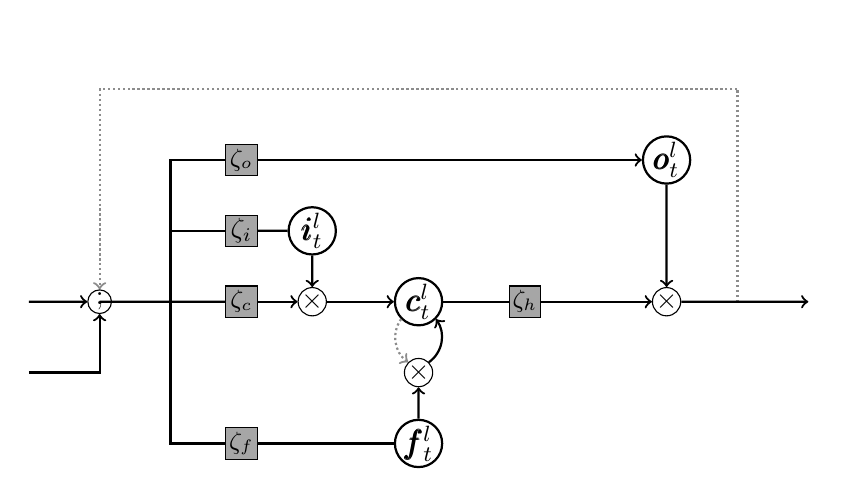
\begin{tikzpicture}[scale=0.45]
		%-------------------------------------------------------------------------------
		% LSTM
		%-------------------------------------------------------------------------------
		\node[circle, inner sep=0pt,minimum size=3mm,fill=white] (conc) 
			at (-0,6) {\textcolor{mDarkTeal}{$;$}};
		
		% outer box
		\draw[densely dotted, thick, gray!90] (18,6) -| (18,12);
		\draw[densely dotted, thick,->, gray!90] (18,12) -| (conc);
		%\draw[thick] (0,0) |- (18,12);
		%\draw[thick] (18,12) |- (0,0);
		
		% core nodes
		\node[circle, draw=black, inner sep=0pt,minimum size=3mm,fill=white] (conc) 
			at (-0,6) {\textcolor{black}{$;$}};
		\node[circle, draw=black, thick, inner sep=0pt,minimum size=6mm,fill=white] (s) 
			at (9,6) {\large\textcolor{black}{$\Cc_t^l$}};
		\node[circle, draw=black, inner sep=0pt,minimum size=3mm,fill=white] (fx) 
			at (9,4) {\textcolor{black}{$\times$}};
		\node[circle, draw=black, thick, inner sep=0pt,minimum size=6mm,fill=white] (f) 
			at (9,2) {\large\textcolor{black}{$\ff_t^l$}};
		\node[circle, draw=black, thick, inner sep=0pt,minimum size=6mm,fill=white] (i) 
			at (6,8) {\large\textcolor{black}{$\ii_t^l$}};
		\node[circle, draw=black, inner sep=0pt,minimum size=3mm,fill=white] (ix) 
			at (6,6) {\textcolor{black}{$\times$}};
		\node[rectangle, draw=black, inner sep=0pt,minimum size=4mm,fill=gray!70] (id) 
			at (4,8) {\textcolor{black}{$\zeta_i$}};
		\node[rectangle, draw=black, inner sep=0pt,minimum size=4mm,fill=gray!70] (sd) 
			at  (4,6) {\small\textcolor{black}{$\zeta_c$}};
		\node[circle, draw=black, thick, inner sep=0pt,minimum size=6mm,fill=white] (o) 
			at (16,10) {\large\textcolor{black}{$\oo_t^l$}};
		\node[circle, draw=black, inner sep=0pt,minimum size=3mm,fill=white] (ox) 
			at (16,6) {\textcolor{black}{$\times$}};
		\node[rectangle, draw=black, inner sep=0pt,minimum size=4mm,fill=gray!70] (hd) 
			at (12,6) {\small\textcolor{black}{$\zeta_h$}};
		\node[rectangle, draw=black, inner sep=0pt,minimum size=4mm,fill=gray!70] (odd) 
			at (4,10) {\small\textcolor{black}{$\zeta_o$}};
		\node[rectangle, draw=black, inner sep=0pt,minimum size=4mm,fill=gray!70] (fd) 
			at (4,2) {\small\textcolor{black}{$\zeta_f$}};
		% recurrency
		\draw (f) edge[thick] (fd);
		\draw[thick] (fd) -| (2,6);
		\draw[thick] (2,6) |- (odd);
		\draw (odd) edge[->,thick] (o);
		\draw[thick] (2,6) |- (id);
		\draw (id) edge[thick] (i);
		% gates
		\draw (o) edge[->, thick] (ox);
		\draw (i) edge[->, thick] (ix);
		\draw (s) edge[->,bend right=45, thick, densely dotted, gray!90] (fx);
		\draw (s) edge[<-,bend left=45, thick] (fx);
		\draw (f) edge[->, thick] (fx);
		% forward
		\draw (-2,4)[->,thick] -| (conc);
		\draw(-2,6) edge[thick,->] (conc);
		\draw (0,6) edge[thick] (sd);
		\draw (sd) edge[->, thick] (ix);
		\draw (ix) edge[->, thick] (s);
		\draw (s) edge[thick] (hd);
		\draw (hd) edge[->, thick] (ox);
		\draw (ox) edge[->, thick] (20,6);
		
		% labels
%		\node[label=above:$\textcolor{white}{\mathcal{I}}$] (we) at (1,6) {};		
		\node[label=below:$\textcolor{white}{\hh_t^{l-1}}$] (ht1) at (-1,4) {};
		\node[label=above:$\textcolor{white}{\xx_t}$] (x) at (-1,6) {};
		\node[label=above:$\textcolor{white}{\hh_t^l}$] (ht) at (19.5,6) {};
		\node[label=above:$\textcolor{white}{\hh_{t-1}^l}$] (x) at (9,12) {};
		\end{tikzpicture}
		\end{figure}
\end{frame}

\begin{frame}{Controller: Signal-Flow (2/2)}
	\alert{LSTM Network} (multiple layers)
	\begin{itemize}
	\item	\alert{Input}: $\xx_t$\\
	\item	\alert{Output}: $[\hh_t^1;\hh_t^2;\dots\hh_t^L]$\\	
	\end{itemize}
	\pause
	\begin{figure}
	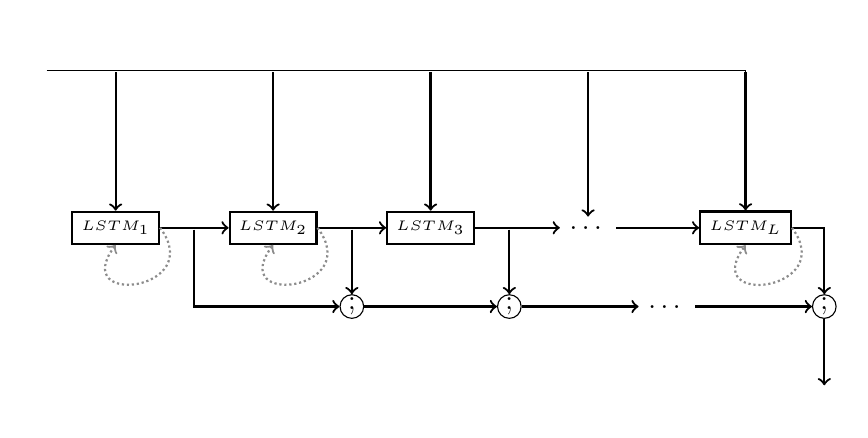
\begin{tikzpicture}[scale=1]
	\tikzset{miniLSTM/.style={draw=black, fill=white, minimum width=20pt, minimum height=10pt, thick}}
	\tikzset{split/.style={circle, draw=black,inner sep=0pt, minimum size = 3mm, fill=white}}
		\node (dummy_node) at (1,0) {};
		\foreach \name/\x in {x1/2, x2/4, x3/6, xd/8, xL/10} {\node[inner sep=0] (\name) at (\x,0) {};}
		\foreach \name/\x in {h1/3, h2/5, h3/7, hL/10} {\node[inner sep=0] (\name) at (\x, -2) {};}
		\foreach \name/\x in {s1/5, s2/7, sL/11} {\node[split] (\name) at (\x,-3) {$\textcolor{black}{\tiny;}$};}
		\foreach \name/\x/\tag in {L1/2/$LSTM_1$, L2/4/$LSTM_2$, L3/6/$LSTM_3$, LL/10/$LSTM_L$} 
		{\node[miniLSTM] (\name) at (\x,-2) {\textcolor{black}{\tiny\tag}};}
		\node (Ld) at (8,-2) {$\dots$};
		\node (sd) at (9,-3) {$\dots$};
		\draw (dummy_node) -| (LL);
		\draw (L1) edge[->,thick] (L2);
		\draw (L2) edge[->,thick] (L3);
		\draw (L3) edge[->,thick] (Ld);
		\draw (Ld) edge[->,thick] (LL);
		\draw[->,thick] (x1) edge (L1.north);
		\draw[->,thick] (x2) edge (L2.north);
		\draw[->,thick] (x3) edge (L3.north);
		\draw[->,thick] (xL) edge (LL.north);
		\draw[->,thick] (xd) edge (Ld.north);
		%\draw[->,thick] (1,0) |- (s0);
		\draw[->,thick] (h1) |- (s1);
		\draw[->,thick] (h2) edge (s1);
		\draw[->,thick] (h3) edge (s2);
		\draw[->,thick] (s1) edge (s2);
		\draw[->,thick] (s2) edge (sd);
		\draw[->,thick] (sd) edge (sL);
		\draw[->,thick] (LL) -| (sL);		
		\draw[->,thick] (sL) edge (11, -4);
		\draw (L1.east) [->, densely dotted, thick, gray!90] .. controls +(0.6,-0.8) and +(-0.6,-0.8) .. (L1.south);
		\draw (L2.east) [->, densely dotted, thick, gray!90] .. controls +(0.6,-0.8) and +(-0.6,-0.8) .. (L2.south);
		\draw (LL.east) [->, densely dotted, thick, gray!90] .. controls +(0.6,-0.8) and +(-0.6,-0.8) .. (LL.south);
		% labels
		\node[label=above right :$\scriptsize\textcolor{white}{\xx_t}$] (xt) at (1,0) {};
		\node[label=above :$\scriptsize\textcolor{white}{\hh_t^1}$] (xt) at (3,-2) {};
		\node[label=above :$\scriptsize\textcolor{white}{\hh_t^2}$] (xt) at (5,-2) {};
		\node[label=above :$\scriptsize\textcolor{white}{\hh_t^3}$] (xt) at (7,-2) {};
		\node[label=below :$\scriptsize\textcolor{white}{[\hh_t^1;\hh_t^2]}$] (xt) at (6,-3) {};
		\node[label=left :$\scriptsize\textcolor{white}{[\hh_t^1;\hh_t^2;\dots;\hh_t^L]}$] (xt) at (11,-4) {};
	\end{tikzpicture}
	\end{figure}
\end{frame}

\begin{frame}{Controller: Outputs}
	\topskip0pt
	\[
	(\pmb{y}_t,\pmb{\xi}_t)=\mathcal{N}([\xx_1;\dots;\xx_T];\vartheta)
	\]
	\vspace{5pt}
	
	\pause
	\alert{User output} $\pmb{y}_t = W_y[\hh_t^1;\dots;\hh_t^L]$
%	\[
%	\pmb{y}_t = \pmb{\upsilon}_t + W_R[\pmb{r}_t^1;\dots;\pmb{r}_t^R] \tag{\alert{Memory-conditioning}}
%	\]
	
	\pause
	\alert{Interface vector} $\pmb{\xi}_t = W_\xi[\hh_t^1;\dots;\hh_t^L]$
	
	\begin{minipage}{0.49\textwidth}
	\begin{itemize}
		\item Read keys: $\pmb{k}_t^{r,i}$ % \in \mathbb{R}^W$
		\item Read strengths: $\beta_t^{r,i}$ % \in [1,\infty)$
		\item Write key: $\pmb{k}_t^w$ % \in \mathbb{R}^W$	
		\item Write strength: $\beta_t^{w}$ % \in [1,\infty)$
		\item Erase vector: $\pmb{e}_t$ % \in [0,1]^W$	
	\end{itemize}
	\end{minipage}
	\begin{minipage}{0.49\textwidth}
	\begin{itemize}
		\item Write vector: $\pmb{v}_t$ % \in \mathbb{R}^W$
		\item Free gates: $\pmb{\phi}_t^i$ % \in [0,1]$		
		\item Allocation gate: $g_t^a$ % \in [0,1]$
		\item Write gate: $g_t^w$ % \in [0,1]$
		\item Read modes: $\pmb{\pi}_t^i$ % \in \mathcal{S}_3$
	\end{itemize}
	\end{minipage}
%	\begin{equation*}
%	\begin{split}
%	\pmb\xi_t = &[\overbrace{\pmb{k}_t^{r,1};\dots;\pmb{k}_t^{r,R};}^\text{\tiny\alert{read keys}}\
%				\overbrace{\hat{\beta}_t^{r,1};\dots;\hat{\beta}_t^{r,R};}^\text{\tiny\alert{read strengths}}\
%				\overbrace{\pmb{k}_t^w;\ \hat{\beta}_t^w;}^\text{\tiny\alert{write key/strength}} \
%				\overbrace{\hat{\pmb{e}}_t;}^\text{\tiny\alert{erase vector}} \\
%				&\underbrace{\pmb{v}_t;}_\text{\tiny\alert{write vector}} \
%				\underbrace{\hat{\pmb{f}}_t^1;\dots;\hat{\pmb{f}_t^R};}_\text{\tiny\alert{free gates}} \
%				\underbrace{\hat{g}_t^a;\ \hat{g}_t^w;}_\text{\tiny\alert{allocation/write gates}}\
%				\underbrace{\hat{\pmb{\pi}}_t^1;\dots;\hat{\pmb{\pi}}_t^R}_\text{\tiny\alert{read modes}}]
%	\end{split}
%	\end{equation*}
\end{frame}

\begin{frame}{Memory Adressing: Content-Lookup}
	\alert{R read keys} $\pmb{k}^{r,i} \in \mathbb{R}^W,\ i=1\dots R$\\
	\alert{R read strengths} $\beta^{r,i} \in [1,\infty),\ i=1\dots R$\\
	\alert{Write key} $\pmb{k}^{w} \in \mathbb{R}^W$\\
	\alert{Write strength} $\beta^{w} \in [1,\infty)$\\
	
	\pause
	\alert{Matching function} $\mathcal{D}$ comparing memory contents
	
	\pause
	\alert{Weighting function} $\mathcal{C}$ normalizing and sharpening matches
	\[
	\mathcal{C}(M,\pmb{k},\beta)[i]= 
	\frac {exp \{\beta\mathcal{D} (\pmb{k},M[i,:])\} }
	{ \sum_{j}{exp \{\beta\mathcal{D} (\pmb{k},M[j,:]) \}}}
	\]
\end{frame}

\begin{frame}{Memory Adressing: R/W}
	\alert{Attention} dictated by weightings $\pmb{w} \in \mathcal{S}^N$\\
	\alert{Erase vector} $\pmb{e}_t \in [0,1]^W$\\
	\alert{Write vector} $\pmb{v}_t \in \mathbb{R}^W$\\

	\alert{Read operations}
	\begin{align*}
	 \pmb{r}_t^i = M_t^\top\pmb{w}_t^{r,i} \\ 
	\end{align*}
	
	\pause
	\alert{Write operations}
	\begin{align*}
	M_t = \underbrace{M_{t-1} \circ (\pmb{1} - \pmb{w}_t^w\pmb{e}_t^\top)}_{\text{erased memory}} + 
	\underbrace{\pmb{w}_t^w\pmb{v}_t^\top}_{\text{new write}}
	\end{align*}
\end{frame}

\begin{frame}{Memory Adressing: Dynamic Allocation}
	\alert{Free gates} $\pmb{\phi}_t^i \in [0,1]^W$\\
	\alert{Allocation gate} $g_t^a \in [0,1]$\\
	\alert{Write gate} $g_t^w \in [0,1]$\\
	
	\alert{"Free list" scheme}
	\begin{align*}
	\pmb{\psi}_t &= \prod\limits_{i=1}^R (\pmb{1} - \pmb{\phi}_t^iw_{t-1}^{r,i}) \tag{\alert{memory retention}}\\
	u_t &= (\pmb{u}_{t-1} + \pmb{w}_{t-1}^w - \pmb{u}_{t-1} \circ \pmb{w}_{t-1}^w) \circ \pmb{\psi}_t \tag{\alert{usage tracking}}\\
	\end{align*}
	
	\pause
	\alert{Attention shift} 
	\begin{itemize}
	\item Obtain the \alert{allocation vector} $\pmb{a}_t$ by normalizing $\pmb{u}_t$\\
	\item \alert{Shift} $\pmb{w}_t$ by $g_t^a\pmb{a}_t$ and \alert{scale} by $g_t^w$
	\end{itemize}
\end{frame}

\begin{frame}{Memory Adressing: Temporal Linking}
	\alert{Read modes}: $\pmb{\pi}_t^i \in \mathcal{S}_3$\\
	
	\pause
	\alert{Temporal Transition} $\pmb{L}_t \in [0,1]^{N\times N}$
	\[
	\pmb{L}[i,j] = \underbrace{(1 - w_t^W[i] - w_t^W[j])\pmb{L}_{t-1}[i,j]}_{\text{\tiny{{Part of last transition}}}} + \underbrace{w_t^w[i]w_{t-1}^w[j]}_{\text{\tiny{Current transition}}}
%	\pmb{p}_t = (1 - \sum\limits_{i}\pmb{w}_t^W[i])\pmb{p}_{t-1} + \pmb{w}_t^W
	\]
	
	\pause
	\alert{Mode Interpolation}
	\[
	\pmb{w}_t^{r,i} = 
					\underbrace{\pmb{\pi}_t^i[1]L\pmb{w}_t^{r,i}}_{\text{\tiny{Forward shift}}} + 
					\underbrace{\pmb{\pi}_t^i[2]\pmb{w}_t^{r,i}}_{\text{\tiny{No shift}}} + 
					\underbrace{\pmb{\pi}_t^i[3]L^\top\pmb{w}_t^{r,i}}_{\text{\tiny{Backward shift}}} 
	\]
\end{frame}

\begin{frame}{Experiments}
	\begin{itemize}
	\item \alert{Language Tasks}
	\begin{itemize}
	\item Inference
	\item Logical Reasoning
	\end{itemize}
	\pause
	\item \alert{Graph Tasks}
	\begin{itemize}
	\item Network Traversal
	\item Policy Learning
	\end{itemize}
	\end{itemize}
\end{frame}

\begin{frame}{Conclusion}
	\alert{Recap}\\
	\begin{itemize}
	\item We can simulate computation and expand upon it by using differentiable, continuous operations.\\
	\item Simple programs (over complex data structures) can now be automagically inferred.\\
	\end{itemize}
\end{frame}

\begin{frame}{Thank you!}
	\centering
	\alert{Questions?}
\end{frame}

\begin{frame}{Appendix: LSTM Equations}

%	\begin{align}
%	\ii_t^l &= \zeta_i(\mathcal{I}) \tag{\alert{input gate}}\\
%	\ff_t^l &= \zeta_f(\mathcal{I})	\tag{\alert{forget gate}}\\
%	\Cc_t^l &= \ff_t^l\Cc_{t-1}^l + \ii_t^l\zeta_c(\mathcal{I}) \tag{\alert{memory cell}}\\
%	\oo_t^l &= \zeta_o(\mathcal{I})	\tag{\alert{output gate}}\\
%	\hh_t^l &= \oo_t^l\zeta_h(\Cc_t^l)		\tag{\alert{hidden layer}}
%	\end{align}
%	\nonumber \\ 
%	\pmb{\upsilon}_t &= W_y[\hh_t^1;\dots;\hh_t^L]		\tag{\alert{output vector}}\\
%	\pmb{\xi}_t &= W_{\xi}[\hh_t^1;\dots;\hh_t^L]		\tag{\alert{interface vector}}
%	\end{align}
	\begin{align}
	\ii_t^l &= \sigma(W_i^l[\xx_t;\hh_{t-1}^l;\hh_t^{l-1}]+\bb_i^l)   \tag{\alert{input gate}}\\
	\ff_t^l &= \sigma(W_f^l[\xx_t;\hh_{t-1}^l;\hh_t^{l-1}]+\bb_f^l)	\tag{\alert{forget gate}}\\
	\Ss_t^l &= \ff_t^l\Ss_{t-1}^l + \ii_t^ltanh(W_s^l[\xx_t;\hh_{t_1}^l;\hh_t^{l-1}] + \bb_s^l)		\tag{\alert{state}}\\
	\oo_t^l &= \sigma(W_o^l[\xx_t;\hh_{t-1}^l;\hh_t^{l-1}]+\bb_o^l)		\tag{\alert{output gate}}\\
	\hh_t^l &= \oo_t^ltanh(\Ss_t^l)		\tag{\alert{hidden}}\\
	\nonumber \\ 
	\pmb{\upsilon}_t &= W_y[\hh_t^1;\dots;\hh_t^L]		\tag{\alert{output vector}}\\
	\pmb{\xi}_t &= W_{\xi}[\hh_t^1;\dots;\hh_t^L]		\tag{\alert{interface vector}}
	\end{align}
\end{frame}

\begin{frame}{Appendix: Further Reading}
	\begin{minipage}{0.49\textwidth}
	\underline{\alert{Neural Architectures}}
	\begin{itemize}
	\item \alert{Learning to Forget}\\ (Gers, Schmidhuber, Cummins)
	\item \alert{Neural Turing Machines}\\ (Graves, Wayne, Danihelka)
	\item \alert{Entity Networks}\\ (Henaff, Weston, Szlam, Bordes, LeCun)
	\item \alert{End-to-End Memory Networks}\\ (Sukhbaatar, Szlam, Weston, Fergus)	
	%\item \alert{Jointly Learning to Align and Translate}\\ (Bahdanau, Cho, Bengio)
	%\item \alert{Principles of Probabilistic Programming Languages} (Goodman)
	%\item \alert{Backprop as a Functor} (Fong, Spivak, Tuyéras)
	%\item \alert{Formal Methods for Probabilistic Programming} (Selsam, Liang, Dill)
	\end{itemize}
	\end{minipage}
	\begin{minipage}{0.49\textwidth}
	\begin{itemize}	
	\item \alert{Jointly Learning to Align and Translate}\\ (Bahdanau, Cho, Bengio)
	\end{itemize}
	\underline{\alert{Probabilistic Programming}}
	\begin{itemize}
	\item \alert{Principles of Probabilistic Programming Languages} (Goodman)
	\item \alert{Backprop as a Functor} (Fong, Spivak, Tuyéras)
	\item \alert{Formal Methods for Probabilistic Programming} (Selsam, Liang, Dill)
	\end{itemize}
	\end{minipage}
\end{frame}

\end{document}
